\section{Vehicle Stop Frequency}
\label{sec:Results_Stops}

Vehicle–stop frequency is the natural kinematic counterpart to the mean-speed metric discussed in Section~\vref{sec:Results_MeanSpeed}. A decrease in the platoon’s mean speed is expected to be accompanied by a rise in complete halts. Table~\vref{tab:StopFreq} and Figures~\vref{fig:StopFreq_2077}–\vref{fig:StopFreq_3462} therefore replicate the structure of the previous section, yet emphasise discrete stop events rather than continuous velocity.

\subparagraph*{General Behaviour.}

For light and moderate flows ($69$--$1385~\unit{\veh\per\hour}$), both \ac{eco-glosa} and \ac{flow-glosa} \emph{decrease} the stop frequency monotonically as the \ac{mpr} increases. At $138~\unit{\veh\per\hour}$, the HBEFA4-\ac{eco-glosa} controller cuts stops from $0.83$ to $0.08~\unit{\stops\per\veh}$ at $90\%$ \ac{mpr}, a reduction of $90\%$. The \ac{flow-glosa} algorithm achieves a similar reduction, though it typically requires about $10\%$ more penetration to do so, which is consistent with its slightly higher cruise speeds.

\subparagraph*{Incipient Congestion: $2077~\unit{\veh\per\hour}$.}
The frequency of vehicle stops starts at about $1.06$ stops per vehicle in the Standard case, as shown in Figure \vref{fig:StopFreq_2077}. Under the PHEMlight5 emission model, the \ac{eco-glosa} controller's performance at this demand level is complex. It initially records a slight increase in stop frequency to $1.08~\unit{\stops\per\veh}$ at $10\%$ \ac{mpr}, which indicates minor instability at the onset of congestion. However, as the \ac{mpr} increases further, the controller becomes highly effective. It progressively reduces the stop frequency, which ultimately falls to just $0.03~\unit{\stops\per\veh}$ at full penetration, a reduction of over $97\%$ compared to the Standard scenario. Under the HBEFA4 model, \ac{eco-glosa} decreases stops to $1.03~\unit{\stops\per\veh}$ before continuing a consistent downward trend. The \ac{flow-glosa} controller is highly effective here, lowering stops to $0.99~\unit{\stops\per\veh}$ at $10\%$ \ac{mpr} and practically eliminating them (to $0.03~\unit{\stops\per\veh}$) by $90\%$ \ac{mpr}, demonstrating strong queue-suppression capabilities just below the jam threshold.

\begin{figure}[htb]
  \centering
  \begin{subfigure}[b]{0.45\textwidth}
    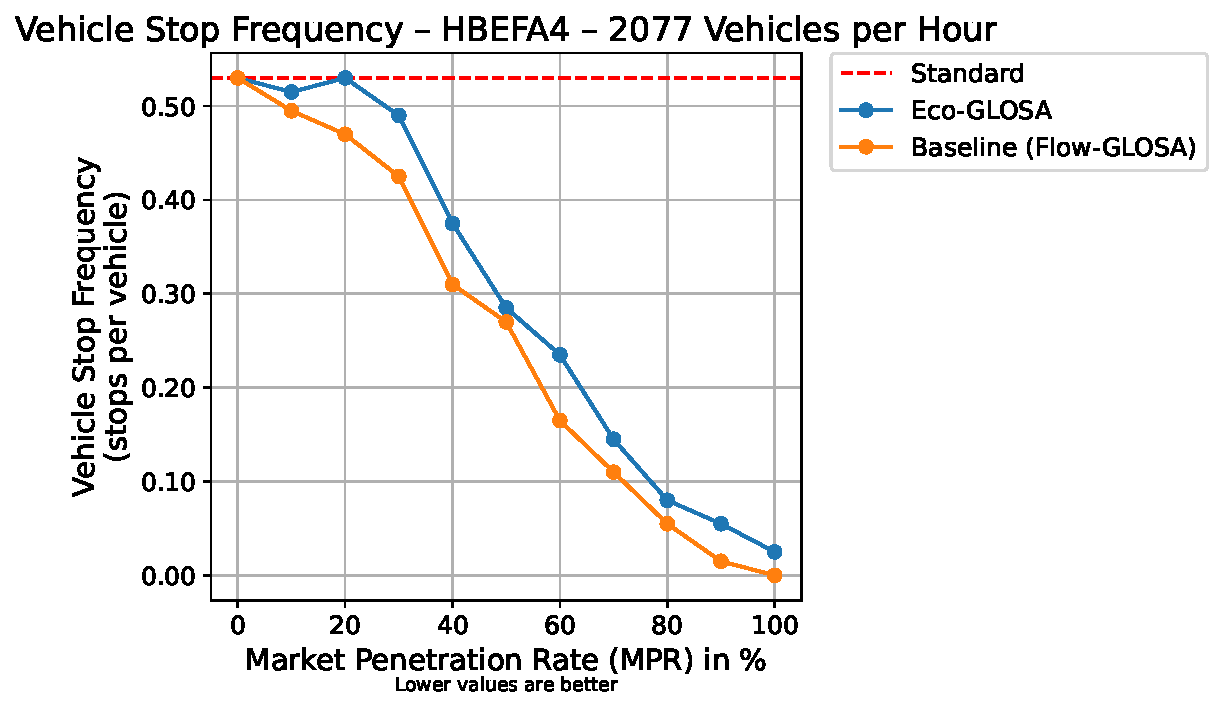
\includegraphics[width=\textwidth]{data/img/VehicleStopFrequency/VehicleStopFrequency_HBEFA4_Cars2077.pdf}
    \caption{Results under the HBEFA4 emission model.}
    \label{fig:StopFreq_2077_HBEFA4}
  \end{subfigure}\hfill
  \begin{subfigure}[b]{0.45\textwidth}
    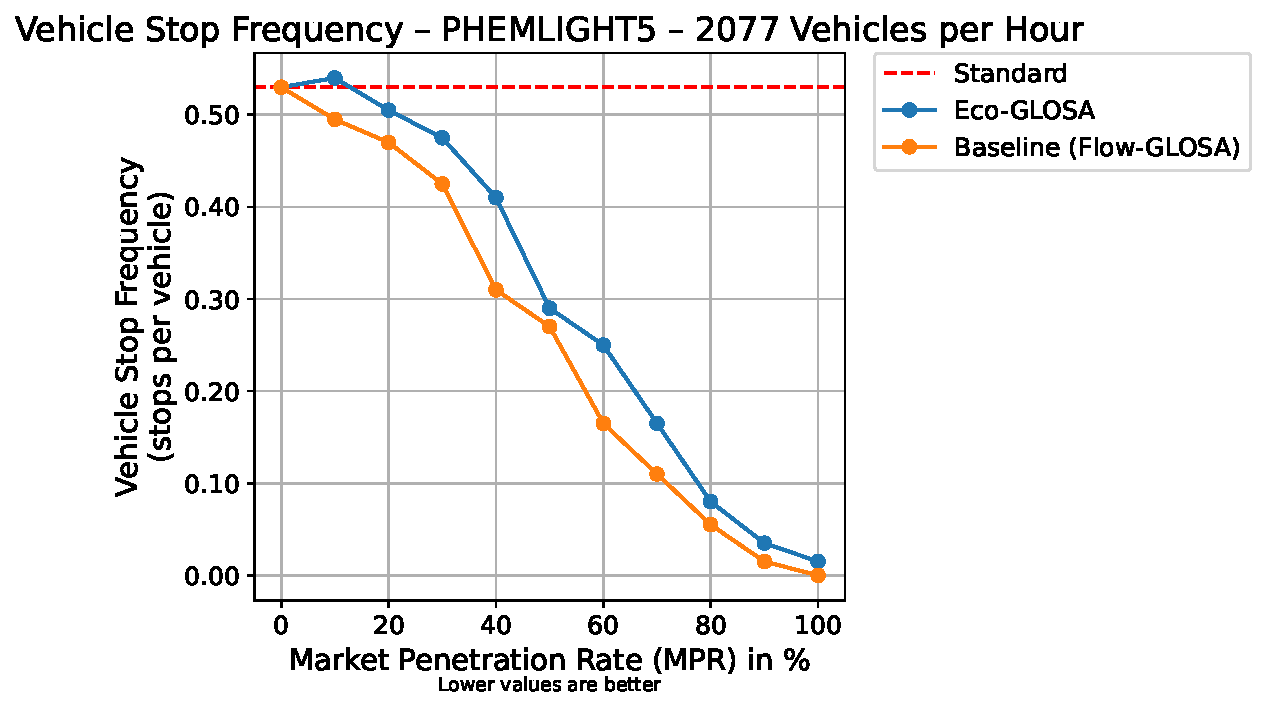
\includegraphics[width=\textwidth]{data/img/VehicleStopFrequency/VehicleStopFrequency_PHEMLIGHT5_Cars2077.pdf}
    \caption{Results under the PHEMlight5 emission model.}
    \label{fig:StopFreq_2077_PHEM}
  \end{subfigure}
  \caption[Vehicle stop frequency vs. \ac{mpr} at $2077~\unit{\veh\per\hour}$]{Vehicle stop frequency versus \ac{mpr} at an incipient congestion level of $2077~\unit{\veh\per\hour}$. The plots compare the Standard, \ac{eco-glosa}, and \ac{flow-glosa} controllers.}
  \label{fig:StopFreq_2077}
\end{figure}

\subparagraph*{Jam Threshold: $2769~\unit{\veh\per\hour}$.}
Figure~\vref{fig:StopFreq_2769} highlights a significant divergence between the two emission models at the jam threshold. With the PHEMlight5 model, the stop frequency for \ac{eco-glosa} increases sharply from its Standard value of $1.36~\unit{\stops\per\veh}$ to $9.53~\unit{\stops\per\veh}$ at just $20\%$ \ac{mpr}. The instability worsens as penetration increases, with the stop count peaking at $23.11~\unit{\stops\per\veh}$ at $90\%$ \ac{mpr}. Although the frequency improves slightly at full penetration, it only falls to $13.16~\unit{\stops\per\veh}$, remaining nearly tenfold higher than the Standard.
\mynewline
The HBEFA4-based \ac{eco-glosa} controller exhibits a different, though still volatile, trend. It remains stable at low penetration before rapidly escalating to $7.74~\unit{\stops\per\veh}$ at $30\%$ \ac{mpr} and reaching a peak of $16.04~\unit{\stops\per\veh}$ at $60\%$. In contrast to the PHEMlight5 result, it then recovers dramatically at higher penetration rates, with stops falling to almost zero ($0.02~\unit{\stops\per\veh}$) at $100\%$ \ac{mpr}.
\mynewline
Throughout this demand level, the \ac{flow-glosa} controller demonstrates its robustness. It maintains a stop frequency at or below $1.28~\unit{\stops\per\veh}$ and declines smoothly to $0.07~\unit{\stops\per\veh}$ at $90\%$, showing strong wave-dampening at the verge of congestion.

\begin{figure}[htb]
  \centering
  \begin{subfigure}[b]{0.45\textwidth}
    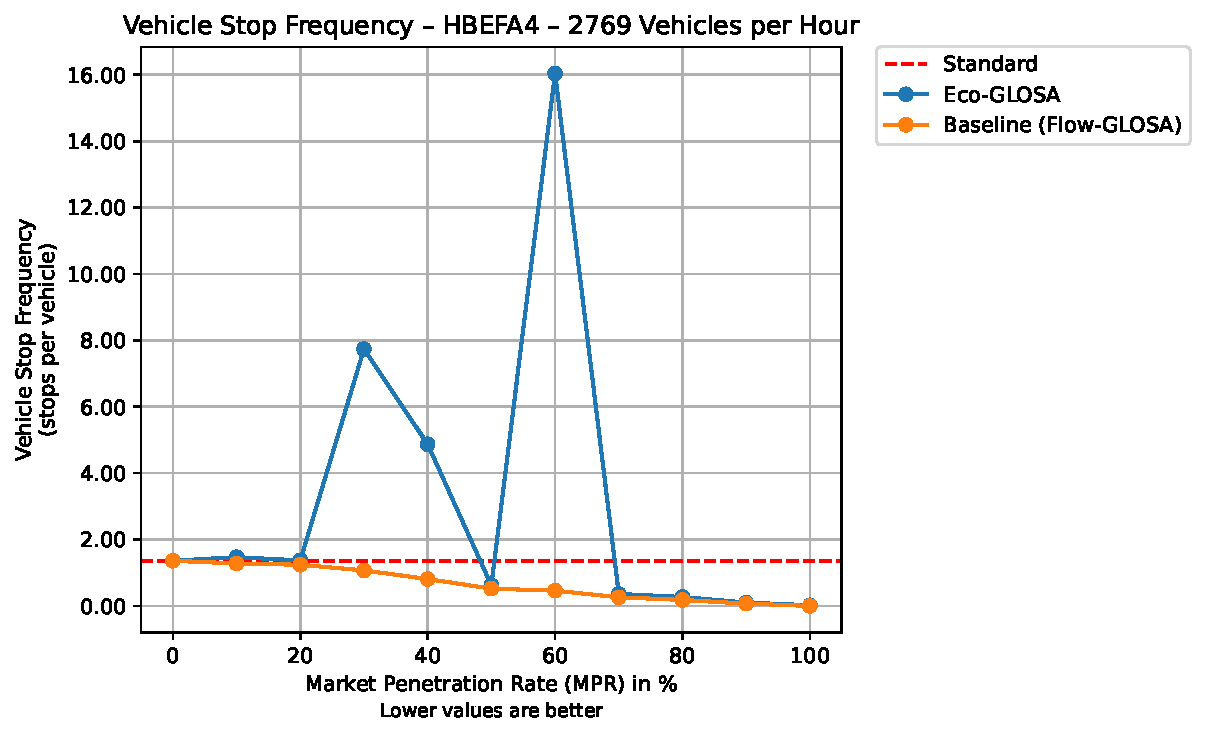
\includegraphics[width=\textwidth]{data/img/VehicleStopFrequency/VehicleStopFrequency_HBEFA4_Cars2769.pdf}
    \caption{Performance with the HBEFA4 emission model.}
    \label{fig:StopFreq_2769_HBEFA4}
  \end{subfigure}\hfill
  \begin{subfigure}[b]{0.45\textwidth}
    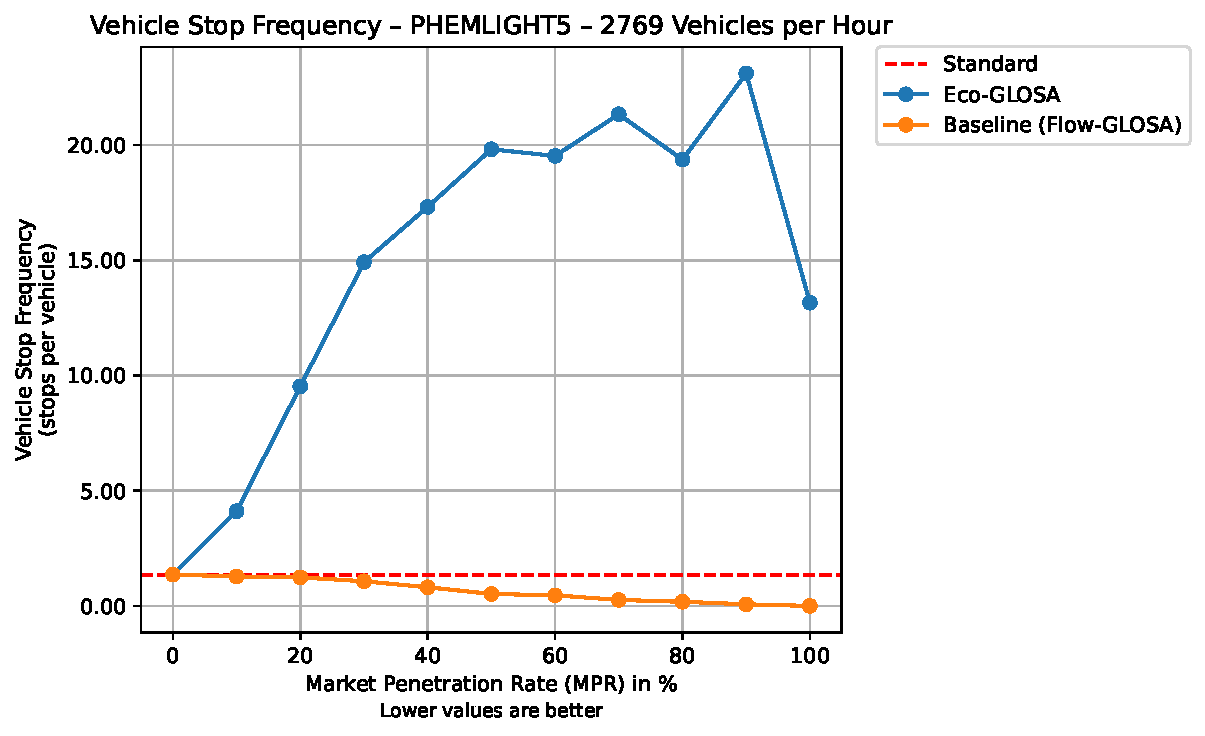
\includegraphics[width=\textwidth]{data/img/VehicleStopFrequency/VehicleStopFrequency_PHEMLIGHT5_Cars2769.pdf}
    \caption{Performance with the PHEMlight5 emission model.}
    \label{fig:StopFreq_2769_PHEM}
  \end{subfigure}
  \caption[Vehicle stop frequency vs. \ac{mpr} at $2769~\unit{\veh\per\hour}$]{Vehicle stop frequency versus \ac{mpr} at the jam threshold of $2769~\unit{\veh\per\hour}$. The plots illustrate the significant performance divergence of the three control strategies.}
  \label{fig:StopFreq_2769}
\end{figure}

\subparagraph*{Full Saturation: $3462~\unit{\veh\per\hour}$.}
The results are displayed in a fully saturated, gridlocked state in Figure~\vref{fig:StopFreq_3462}. Under these conditions, the \ac{eco-glosa} controller fails to improve traffic flow and instead exacerbates congestion. With the HBEFA4 model, its stop frequency shows a generally increasing trend, peaking at $35.14~\unit{\stops\per\veh}$ at an \ac{mpr} of $80\%$. The negative impact is even more pronounced with the PHEMlight5 model, where the stop count reaches a maximum of $38.94~\unit{\stops\per\veh}$ at $100\%$ \ac{mpr}.
\mynewline
Contrastingly, the \ac{flow-glosa} controller exhibits an extraordinary capacity to alleviate congestion. Its effectiveness becomes apparent as penetration increases, with stop frequency dropping sharply beyond an \ac{mpr} of $50\%$. The stop count falls to just $5.28~\unit{\stops\per\veh}$ at $60\%$ \ac{mpr}, then continues to decline to near-zero levels: $0.19$ at $80\%$, $0.05$ at $90\%$, and only $0.01~\unit{\stops\per\veh}$ at full penetration.
\mynewline
This dramatic reduction in stops is indicative of a dissolved queue, a conclusion supported by the simultaneous increase in vehicle speed. The mean speeds under \ac{flow-glosa} climb well above the jam threshold of $4~\unit{\metre\per\second}$, as shown in Figures~\vref{fig:MeanSpeed_HBEFA4_3462} and \vref{fig:MeanSpeed_PHEM_3462}. This confirms that the advisory successfully restores free-flow conditions once a critical penetration is reached. At extreme demand, \ac{flow-glosa} not only prevents further stops but actively resolves the gridlock, demonstrating its capacity to recover throughput under severe saturation.

\begin{figure}[htb]
  \centering
  \begin{subfigure}[b]{0.45\textwidth}
    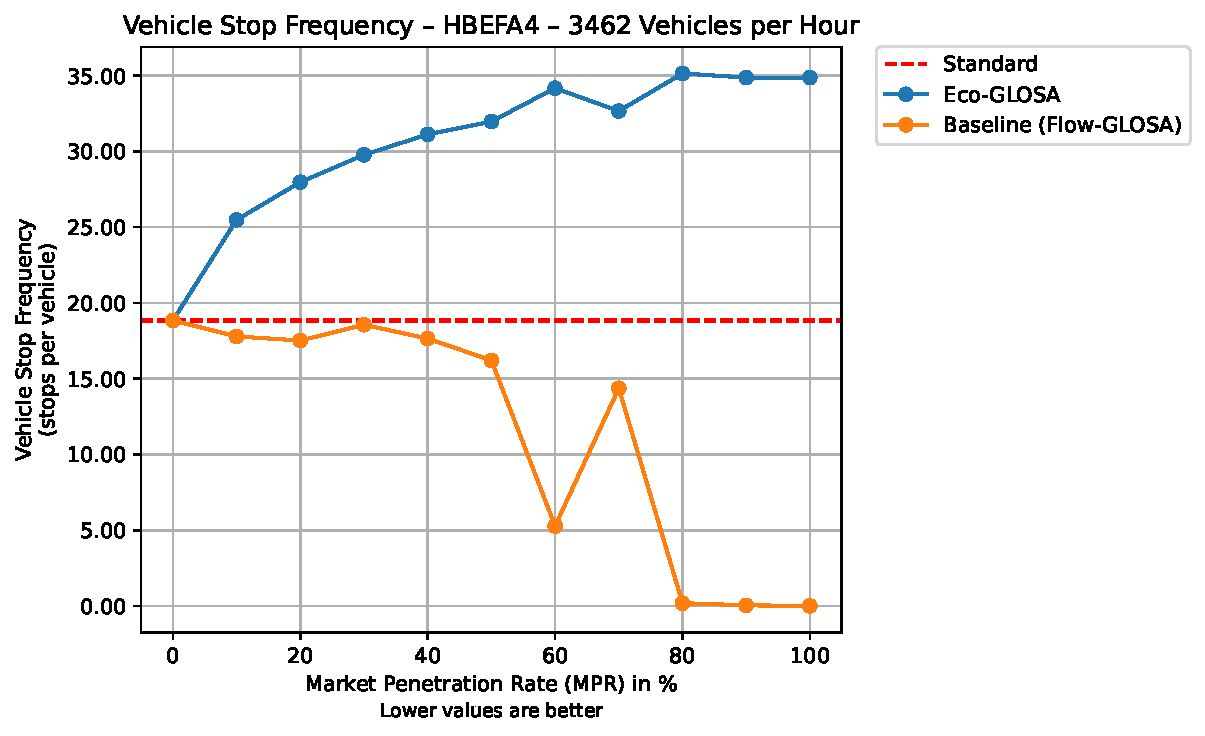
\includegraphics[width=\textwidth]{data/img/VehicleStopFrequency/VehicleStopFrequency_HBEFA4_Cars3462.pdf}
    \caption{Simulation results using the HBEFA4 model.}
    \label{fig:StopFreq_3462_HBEFA4}
  \end{subfigure}\hfill
  \begin{subfigure}[b]{0.45\textwidth}
    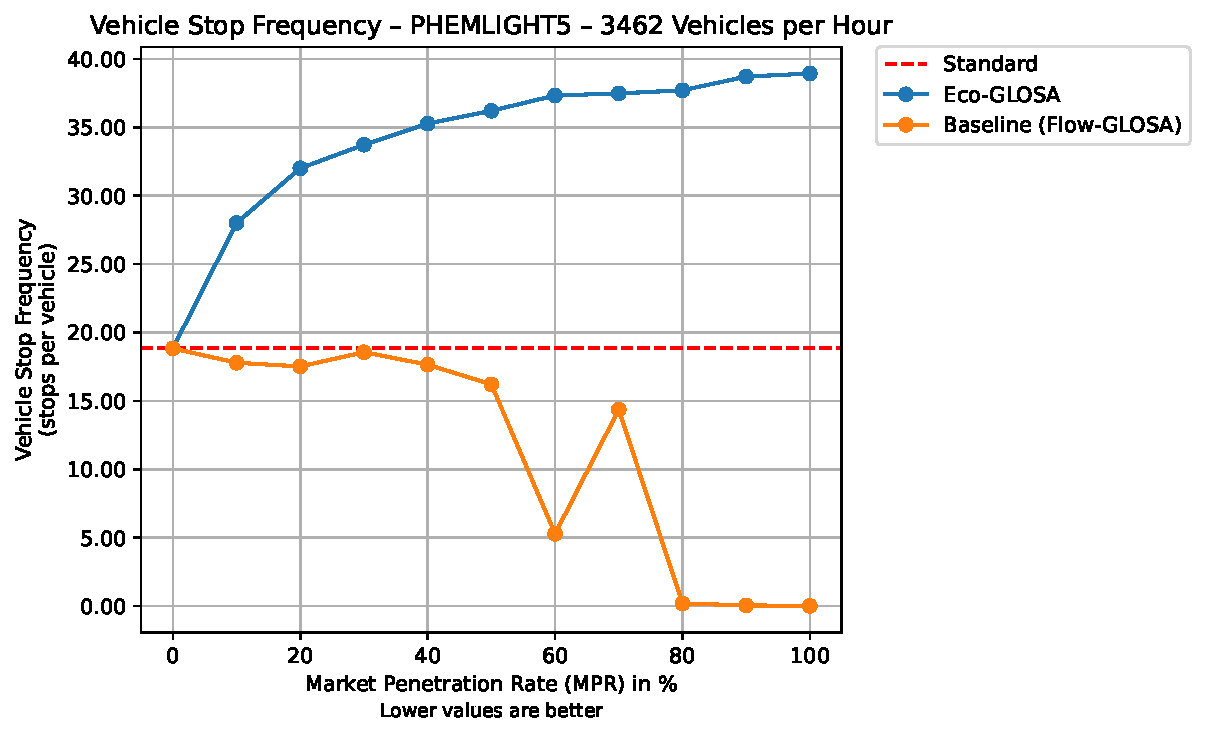
\includegraphics[width=\textwidth]{data/img/VehicleStopFrequency/VehicleStopFrequency_PHEMLIGHT5_Cars3462.pdf}
    \caption{Simulation results using the PHEMlight5 model.}
    \label{fig:StopFreq_3462_PHEM}
  \end{subfigure}
  \caption[Vehicle stop frequency vs. \ac{mpr} at $3462~\unit{\veh\per\hour}$]{Vehicle stop frequency as a function of \ac{mpr} in the fully saturated regime of $3462~\unit{\veh\per\hour}$. The outcomes for the Standard, \ac{eco-glosa}, and \ac{flow-glosa} controllers are shown.}
  \label{fig:StopFreq_3462}
\end{figure}

\subparagraph*{Key Takeaways.}
\begin{enumerate}[label=(\alph*)]
    \item In light to moderate demand scenarios ($69$--$1385~\unit{\veh\per\hour}$), both controllers effectively reduce stop frequency as the \ac{mpr} increases. The \ac{eco-glosa} strategy proves particularly effective, achieving up to a $90\%$ reduction in stops at high penetration rates.
    
    \item As congestion begins to form ($2077~\unit{\veh\per\hour}$), the \ac{flow-glosa} controller demonstrates superior stop suppression, nearly eliminating them at high \ac{mpr}. In contrast, the \ac{eco-glosa} controller exhibits minor instability at low penetration before its effectiveness improves at higher penetration levels.
    
    \item At the jam threshold ($2769~\unit{\veh\per\hour}$), the \ac{eco-glosa} controller's performance degrades significantly, leading to runaway stop counts that exceed $20~\unit{\stops\per\veh}$. Conversely, the \ac{flow-glosa} controller remains stable, keeping the stop frequency at or below $1.3~\unit{\stops\per\veh}$.
    
    \item In fully saturated conditions ($3462~\unit{\veh\per\hour}$), only the \ac{flow-glosa} strategy is capable of resolving the gridlock. At an \ac{mpr} above $80\%$, it drives stop counts to near zero while restoring mean speeds above the $4~\unit{\metre\per\second}$ jam threshold. Meanwhile, the \ac{eco-glosa} strategy accumulates over $35~\unit{\stops\per\veh}$.
    
    \item The combined analysis of stop frequency and mean speed is crucial. This dual-metric approach distinguishes true gridlock resolution, as achieved by \ac{flow-glosa}, from misleading \enquote{zero-stop} scenarios where vehicles might simply be immobile within a queue.
\end{enumerate}

\begin{table}[htb]
  \centering
  \caption[Vehicle stop frequency for all traffic volumes and \ac{mpr} values]{Vehicle stop frequency, measured in $\unit{\stops\per\veh}$, tabulated for all traffic volumes and \ac{mpr} values. Data is provided for the Standard, \ac{flow-glosa}, and \ac{eco-glosa} controllers under both the HBEFA4 and PHEMlight5 emission models.}
  \label{tab:StopFreq}
  \resizebox{\textwidth}{!}{%
  \begin{tabular}{r l l r *{10}{r}}
    \toprule
    Vehicles & Algorithm & Fuel Model & \textbf{0\% (Standard)} & 10\% & 20\% & 30\% & 40\% & 50\% & 60\% & 70\% & 80\% & 90\% & 100\%\\
    \midrule
    69  & \ac{eco-glosa} & HBEFA4 & \textbf{0.76} & 0.56 & 0.72 & 0.56 & 0.49 & 0.54 & 0.43 & 0.22 & 0.28 & 0.11 & 0.00\\
    69  & Baseline (\ac{flow-glosa}) & HBEFA4 & \textbf{0.76} & 0.56 & 0.78 & 0.61 & 0.49 & 0.54 & 0.49 & 0.22 & 0.28 & 0.17 & 0.00\\
    69  & \ac{eco-glosa} & PHEMLIGHT5 & \textbf{0.76} & 0.56 & 0.72 & 0.50 & 0.49 & 0.54 & 0.43 & 0.22 & 0.28 & 0.11 & 0.00\\
    69  & Baseline (\ac{flow-glosa}) & PHEMLIGHT5 & \textbf{0.76} & 0.56 & 0.78 & 0.61 & 0.49 & 0.54 & 0.49 & 0.22 & 0.28 & 0.17 & 0.00\\
    \midrule
    138 & \ac{eco-glosa} & HBEFA4 & \textbf{0.83} & 0.64 & 0.64 & 0.59 & 0.37 & 0.27 & 0.27 & 0.19 & 0.13 & 0.08 & 0.00\\
    138 & Baseline (\ac{flow-glosa}) & HBEFA4 & \textbf{0.83} & 0.61 & 0.62 & 0.59 & 0.37 & 0.32 & 0.24 & 0.16 & 0.16 & 0.05 & 0.00\\
    138 & \ac{eco-glosa} & PHEMLIGHT5 & \textbf{0.83} & 0.67 & 0.56 & 0.59 & 0.37 & 0.29 & 0.16 & 0.19 & 0.13 & 0.08 & 0.00\\
    138 & Baseline (\ac{flow-glosa}) & PHEMLIGHT5 & \textbf{0.83} & 0.61 & 0.62 & 0.59 & 0.37 & 0.32 & 0.24 & 0.16 & 0.16 & 0.05 & 0.00\\
    \midrule
    346 & \ac{eco-glosa} & HBEFA4 & \textbf{0.76} & 0.68 & 0.65 & 0.51 & 0.47 & 0.38 & 0.28 & 0.27 & 0.19 & 0.08 & 0.01\\
    346 & Baseline (\ac{flow-glosa}) & HBEFA4 & \textbf{0.76} & 0.69 & 0.64 & 0.49 & 0.44 & 0.36 & 0.24 & 0.27 & 0.15 & 0.06 & 0.00\\
    346 & \ac{eco-glosa} & PHEMLIGHT5 & \textbf{0.76} & 0.65 & 0.73 & 0.56 & 0.51 & 0.35 & 0.31 & 0.27 & 0.17 & 0.07 & 0.03\\
    346 & Baseline (\ac{flow-glosa}) & PHEMLIGHT5 & \textbf{0.76} & 0.69 & 0.64 & 0.49 & 0.44 & 0.36 & 0.24 & 0.27 & 0.15 & 0.06 & 0.00\\
    \midrule
    692 & \ac{eco-glosa} & HBEFA4 & \textbf{0.79} & 0.78 & 0.62 & 0.54 & 0.45 & 0.42 & 0.23 & 0.26 & 0.16 & 0.06 & 0.01\\
    692 & Baseline (\ac{flow-glosa}) & HBEFA4 & \textbf{0.79} & 0.70 & 0.63 & 0.53 & 0.45 & 0.37 & 0.23 & 0.22 & 0.13 & 0.05 & 0.01\\
    692 & \ac{eco-glosa} & PHEMLIGHT5 & \textbf{0.79} & 0.69 & 0.66 & 0.60 & 0.50 & 0.41 & 0.29 & 0.25 & 0.20 & 0.05 & 0.01\\
    692 & Baseline (\ac{flow-glosa}) & PHEMLIGHT5 & \textbf{0.79} & 0.70 & 0.63 & 0.53 & 0.45 & 0.37 & 0.23 & 0.22 & 0.13 & 0.05 & 0.01\\
    \midrule
    1385 & \ac{eco-glosa} & HBEFA4 & \textbf{0.91} & 0.90 & 0.82 & 0.69 & 0.58 & 0.46 & 0.41 & 0.25 & 0.19 & 0.10 & 0.02\\
    1385 & Baseline (\ac{flow-glosa}) & HBEFA4 & \textbf{0.91} & 0.84 & 0.79 & 0.70 & 0.55 & 0.40 & 0.31 & 0.21 & 0.13 & 0.08 & 0.00\\
    1385 & \ac{eco-glosa} & PHEMLIGHT5 & \textbf{0.91} & 0.89 & 0.81 & 0.75 & 0.57 & 0.43 & 0.43 & 0.22 & 0.22 & 0.09 & 0.05\\
    1385 & Baseline (\ac{flow-glosa}) & PHEMLIGHT5 & \textbf{0.91} & 0.84 & 0.79 & 0.70 & 0.55 & 0.40 & 0.31 & 0.21 & 0.13 & 0.08 & 0.00\\
    \midrule
    2077 & \ac{eco-glosa} & HBEFA4 & \textbf{1.06} & 1.03 & 1.06 & 0.98 & 0.75 & 0.57 & 0.47 & 0.29 & 0.16 & 0.11 & 0.05\\
    2077 & Baseline (\ac{flow-glosa}) & HBEFA4 & \textbf{1.06} & 0.99 & 0.94 & 0.85 & 0.62 & 0.54 & 0.33 & 0.22 & 0.11 & 0.03 & 0.00\\
    2077 & \ac{eco-glosa} & PHEMLIGHT5 & \textbf{1.06} & 1.08 & 1.01 & 0.95 & 0.82 & 0.58 & 0.50 & 0.33 & 0.16 & 0.07 & 0.03\\
    2077 & Baseline (\ac{flow-glosa}) & PHEMLIGHT5 & \textbf{1.06} & 0.99 & 0.94 & 0.85 & 0.62 & 0.54 & 0.33 & 0.22 & 0.11 & 0.03 & 0.00\\
    \midrule
    \textbf{2769} & \textbf{\ac{eco-glosa}} & \textbf{HBEFA4} & \textbf{1.36} & \textbf{1.47} & \textbf{1.37} & \textbf{7.74} & \textbf{4.87} & \textbf{0.62} & \textbf{16.04} & \textbf{0.36} & \textbf{0.27} & \textbf{0.10} & \textbf{0.02}\\
    2769 & Baseline (\ac{flow-glosa}) & HBEFA4 & \textbf{1.36} & 1.28 & 1.24 & 1.07 & 0.81 & 0.52 & 0.46 & 0.26 & 0.18 & 0.07 & 0.00\\
    \textbf{2769} & \textbf{\ac{eco-glosa}} & \textbf{PHEMLIGHT5} & \textbf{1.36} & \textbf{4.11} & \textbf{9.53} & \textbf{14.92} & \textbf{17.32} & \textbf{19.82} & \textbf{19.53} & \textbf{21.34} & \textbf{19.37} & \textbf{23.11} & \textbf{13.16}\\
    2769 & Baseline (\ac{flow-glosa}) & PHEMLIGHT5 & \textbf{1.36} & 1.28 & 1.24 & 1.07 & 0.81 & 0.52 & 0.46 & 0.26 & 0.18 & 0.07 & 0.00\\
    \midrule
    \textbf{3462} & \textbf{\ac{eco-glosa}} & \textbf{HBEFA4} & \textbf{18.84} & \textbf{25.48} & \textbf{27.97} & \textbf{29.77} & \textbf{31.12} & \textbf{31.97} & \textbf{34.17} & \textbf{32.66} & \textbf{35.14} & \textbf{34.87} & \textbf{34.87}\\
    3462 & Baseline (\ac{flow-glosa}) & HBEFA4 & \textbf{18.84} & 17.79 & 17.52 & 18.56 & 17.65 & 16.21 & 5.28 & 14.37 & \textbf{0.19} & \textbf{0.05} & \textbf{0.01}\\
    \textbf{3462} & \textbf{\ac{eco-glosa}} & \textbf{PHEMLIGHT5} & \textbf{18.84} & \textbf{28.01} & \textbf{32.01} & \textbf{33.73} & \textbf{35.27} & \textbf{36.21} & \textbf{37.33} & \textbf{37.48} & \textbf{37.71} & \textbf{38.71} & \textbf{38.94}\\
    3462 & Baseline (\ac{flow-glosa}) & PHEMLIGHT5 & \textbf{18.84} & 17.79 & 17.52 & 18.56 & 17.65 & 16.21 & 5.28 & 14.37 & \textbf{0.19} & \textbf{0.05} & \textbf{0.01}\\
    \bottomrule
  \end{tabular}}
\end{table}